% Using Free and Open Source Solutions in Geospatial Science Education
% This work by Vaclav Petras is licensed under
% a Creative Commons Attribution-ShareAlike 4.0 International License.

\documentclass[xcolor={dvipsnames,usenames},beamer]{beamer}
% ,handout,notes=show
% ,aspectratio=169

\makeatletter
\def\beamer@framenotesbegin{% at beginning of slide
  \gdef\beamer@noteitems{}%
  \gdef\beamer@notes{{}}% used to be totally empty.
}
\makeatother

\usepackage{textcomp}
\usepackage[utf8]{inputenc}
\usepackage[american]{babel}
\usepackage{graphicx}
\usepackage{url}

\usepackage{tikz}
\usetikzlibrary{arrows,shapes,spy,calc}

\tikzstyle{every picture}+=[remember picture]
\tikzstyle{na} = [baseline=-.5ex]

% frames have to be fragile
\newif\ifnotes
% \input{tmpnotessettings}
% \notestrue


\ifnotes
\setbeamertemplate{note page}[plain]
% \setbeamertemplate{note page}[compress]
\setbeamerfont{note page}{size=\large}
% \setbeameroption{show only notes}
\setbeameroption{show notes}
\usepackage{pgfpages}
\pgfpagesuselayout{2 on 1}[a4paper,border shrink=5mm]%
\else
%\setbeameroption{hide notes}
\fi
%\notesfalse

\usepackage[absolute,overlay]{textpos}

\usepackage{listings}


% \usetheme{Warsaw}
\usetheme{Madrid}
% \usetheme{Frankfurt}
% \useoutertheme{infolines}
\usecolortheme[named=MidnightBlue]{structure}
% \usecolortheme[named=PineGreen]{structure}
\setbeamertemplate{navigation symbols}{}

\setbeamertemplate{itemize items}[default]
\setbeamertemplate{enumerate items}[default]
% \useinnertheme{rectangles}
\setbeamertemplate{blocks}[default]


%%%%%%%%%%%%%%%%%%%%%%%%%%%%%%%%%%%%%%%%%%%%%%%%%%%%%%%%%%%%%%%%%%%%
%%%%%%%%%%%%%%%%%%%%%%%%%%%%%%%%%%%%%%%%%%%%%%%%%%%%%%%%%%%%%%%%%%%%

% \newcommand{\n}[1]{$^{\color{gray}{\mbox{\tiny#1}}}$}
\newcommand{\n}[1]{$^{\textcolor{gray}{\mbox{\tiny{#1}}}}$}

%%%%%%%%%%%%%%%%%%%%%%%%%%%%%%%%%%%%%%%%%%%%%%%%%%%%%%%%%%%%%%%%%%%%
%%%%%%%%%%%%%%%%%%%%%%%%%%%%%%%%%%%%%%%%%%%%%%%%%%%%%%%%%%%%%%%%%%%%

\title[FOSS4G in education]
{Using Free and Open Source Solutions \mbox{in Geospatial Science Education}}
\subtitle{Tools and ideas for better geospatial science education}
%\pdforstring{}{}

\author[Vaclav Petras]
{Vaclav Petras (Vashek)\n{1}\\
{\scriptsize
Anna Petrasova\n{1},
Keren Cepero-Perez\n{1},
Markus Neteler\n{2},
\mbox{
Luca Delucchi\n{2},
Martin Landa\n{3},
Helena Mitasova\n{1}
}
}
}

\institute[NC State University]
{%
$^1$North Carolina State University \\
$^2$Fondazione Edmund Mach\\
$^3$Czech Technical University in Prague and GISMentors
% Center for Geospatial Analytics \\
}

\date[FOSS4G Europe 2015]{July 16, 2015\\
  \href{http://europe.foss4g.org/2015/}{FOSS4G Europe}}

\setbeamercovered{transparent}

\hypersetup{%
 pdfauthor={Vaclav Petras},%
 pdfsubject={FOSS4G Europe 2015},%
 pdfkeywords={sample data} {teaching} {free software} {open science}
   {open education} {geospatial modeling} {GRASS GIS}
}

\newcommand{\overovaciref}[1]{{\scriptsize(\ref{#1})}}


\usepackage{tipa}
\newcommand{\pron}[2]{#1 [#2]}


\newcommand{\beginbackup}{
  \newcounter{framenumbervorappendix}
  \setcounter{framenumbervorappendix}{\value{framenumber}}
}
\newcommand{\backupend}{
  \addtocounter{framenumbervorappendix}{-\value{framenumber}}
  \addtocounter{framenumber}{\value{framenumbervorappendix}}
}


%%%%%%%%%%%%%%%%%%%%%%%%%%%%%%%%%%%%%%%%%%%%%%%%%%%%%%%%%%%%%%%%%%%%
%%%%%%%%%%%%%%%%%%%%%%%%%%%%%%%%%%%%%%%%%%%%%%%%%%%%%%%%%%%%%%%%%%%%
%%%%%%%%%%%%%%%%%%%%%%%%%%%%%%%%%%%%%%%%%%%%%%%%%%%%%%%%%%%%%%%%%%%%
%%%%%%%%%%%%%%%%%%%%%%%%%%%%%%%%%%%%%%%%%%%%%%%%%%%%%%%%%%%%%%%%%%%%
\begin{document}

\newcommand{\logowidth}{1.0em}
\newcommand{\logospace}{\hspace{0.2em}}
\newcommand{\includecclogo}[1]{\includegraphics[width=\logowidth]{./images/logos/#1}}

%%%%%%%%%%%%%%%%%%%%%%%%%%%%%%%%%%%%%%%%%%%%%%%%%%%%%%%%%%%%%%%%%%%%
\frame{
\titlepage
\begin{center}
\href{http://creativecommons.org/licenses/by-sa/4.0/}{
\includecclogo{cc}
\logospace
\includecclogo{by}
\logospace
\includecclogo{sa}
}
\end{center}
}

\newcommand{\quoteTitle}[3]{%
  \href{#3}%
    {\emph{#1}\\%
    \hfill%
    {\footnotesize#2}%
    \smallskip}%
  }
\newcommand{\quoteText}[3]{\quoteTitle{#1}{#2}{#3}}

\begingroup
\setbeamertemplate{background}{%
\begin{minipage}{\paperwidth}
  \centering
  \rule{0px}{0.15\textheight}\\%
  
\includegraphics[height=0.8\textheight]{./images/general/growing}%
\end{minipage}
}
%%%%%%%%%%%%%%%%%%%%%%%%%%%%%%%%%%%%%%%%%%%%%%%%%%%%%%%%%%%%%%%%%%%%%
\begin{frame}{Free and open source software}

\quoteTitle{Open Source Software Is Now a Norm in Businesses}%
  {Katherine Noyes, PCWorld, May 18, 2011}%
  {http://www.pcworld.com/article/228136/open_source_software_now_a_norm_in_businesses.html}

\quoteTitle{Open Source has Become Mainstream but Still Drives Innovation}%
  {Talend Yves de Montcheuil, ZDNet, May 2, 2012}%
  {http://www.zdnet.com/article/open-source-has-become-mainstream-but-still-drives-innovation/}

% Along with every large telecoms provider 10 of Europe's 15 largest banks are
% now running projects on Postgres.
\quoteText{10 of Europe's 15 largest banks are now running [...] Postgres}%
  {Sandor Klein said for ZDNet (Toby Wolpe), November 19, 2013}%
  {http://www.zdnet.com/article/oracle-database-costs-are-driving-firms-to-postgres-says-enterprisedb/}

\quoteTitle{Redmond top man Satya Nadella: 'Microsoft loves Linux'}%
  {Neil McAllister, The Register, October 20, 2014}%
  {http://www.theregister.co.uk/2014/10/20/microsoft_cloud_event/}

\quoteTitle{Survey indicates four out of five developers now use open source}%
  {Steven J. Vaughan-Nichols, ZDNet, October 29, 2014}%
  {http://www.zdnet.com/article/survey-indicates-four-out-of-five-developers-now-use-open-source/}
% This popularity, said Hammond, means that "open source is taking over.
% This is a golden age for developers." A consequence from this is that
% "We are now seeing open source tech compete with open source tech;
% it's no longer open-source software vs proprietary."
% (Jeffrey Hammond, a Forrester Research VP and Principal Analyst,
% At the All Things Open conference 2014)
% 80% of developers used open source in past 12 months, 99% in India and China,
% numbers greater for students in general (personal notes from talk at All Things Open)
  
\quoteText{64\% of internet exchange points are now using\,[...]\,an open source solution}%
  {Gijs Hillenius, Joinup Open source observatory, June 8, 2015}%
  {https://joinup.ec.europa.eu/community/osor/news/2/3-internet-exchange-points-use-czech-open-source-router}
% 2/3 Internet Exchange Points use Czech open source router
% Almost two-thirds (64 per cent) of Internet Exchange Points are now using BIRD,
% an open source router solution maintained by the Czech CZ.NIC Association,
% taking first place from proprietary routers.

\quoteTitle{Open Sourcing Is No Longer Optional, Not Even for Apple}%
  {Klint Finley, WIRED, June 9, 2015}%
  {http://www.wired.com/2015/06/open-sourcing-no-longer-optional-not-even-apple/}

% ``Red Hat Enterprise Linux alone, runs over half the world's equity trading volume''
% http://opensource.com/business/13/1/could-open-source-build-jetliner

% Coverity finds open source software quality better than proprietary code
% By Steven J. Vaughan-Nichols, ZDNet, April 16, 2014
% http://www.zdnet.com/article/coverity-finds-open-source-software-quality-better-than-proprietary-code/

% Docker
% http://www.zdnet.com/article/heres-how-microsoft-is-supporting-the-open-source-docker-container-model/

% Linux kernel devs
% http://www.zdnet.com/blog/open-source/top-five-linux-contributor-microsoft/9254

% .NET
% http://blogs.msdn.com/b/dotnet/archive/2014/11/12/net-core-is-open-source.aspx
% http://opensource.com/business/14/11/microsoft-dot-net-empower-open-source-communities
% http://news.microsoft.com/2014/11/12/microsoft-takes-net-open-source-and-cross-platform-adds-new-development-capabilities-with-visual-studio-2015-net-2015-and-visual-studio-online/
% .NET Foundation with https://github.com/dotnet
% http://www.dotnetfoundation.org/
% Microsoft is providing the full .NET server stack in open source, including ASP.NET,
% the .NET compiler, the .NET Core Runtime, Framework and Libraries,
% enabling developers to build with .NET across Windows, Mac or Linux.
% http://news.microsoft.com/2014/11/12/microsoft-takes-net-open-source-and-cross-platform-adds-new-development-capabilities-with-visual-studio-2015-net-2015-and-visual-studio-online/

% Steve Ballmer proclaiming back in 2001 that "Linux is a cancer."
% In the years since then Microsoft certainly attacked Linux like it was a cancer
% — doing everything from sponsoring SCO's copyright attack on Linux to claiming
% that Linux violated unnamed Microsoft patents to endless FUD assaults.
% After decades of resistance, Microsoft supports a variety of open-source programs
% Microsoft is acutely aware that Azure is the only purely proprietary cloud out here.
% All its competition — Amazon Web Services, Google Compute, OpenStack,
% etc. — all run on Linux and offer Linux server services.
% Nadella admitted that 20 percent of the operating systems on Azure are Linux.
% http://www.zdnet.com/article/why-microsoft-loves-linux/
% https://twitter.com/MSFTnews/status/524262781592539136

% Microsoft's participation in these efforts underscores the fact
% that nothing has changed more in the last couple of decades
% than how software is fundamentally built. Today most software is built collaboratively.
% The very nature of open source development is to accelerate technology,
% which is why competition today is so fierce and things move faster than ever before.
% http://www.linux.com/news/featured-blogs/158-jim-zemlin/795282-microsoft-appeals-to-developers-developers-developers

% As the first major computer company to make Open Source development a key part of its
% ongoing software strategy, Apple remains committed to the Open Source development model.
% Apple uses software created by the Open Source community [...] and returns its enhancements
% to the community.
% Apple believes that using Open Source methodology makes Mac OS X a more robust,
% secure operating system, as its core components have been subjected to the crucible
% of peer review for decades. Any problems found with this software can be immediately
% identified and fixed by Apple and the Open Source community.
% https://www.apple.com/opensource/

% Open source is now pervasive among the developer community, says [analyst Al Hilwa, of IDC]. "This is something that Microsoft cannot ignore."
% http://www.infoworld.com/article/2850050/microsoft-net/microsoft-open-source-net-cant-match-open-source-java.html

\end{frame}
\endgroup

%%%%%%%%%%%%%%%%%%%%%%%%%%%%%%%%%%%%%%%%%%%%%%%%%%%%%%%%%%%%%%%%%%%%%
\begin{frame}{Free and open source software}

% science
\quoteText{Software [...] developed as part of novel methods is as 
    important for the method's implementation [...]
    Such software [...] must be made available to readers upon publication.}
  {Social software, Nature Methods 4, 189, 2007}%
  {http://www.nature.com/nmeth/journal/v4/n3/full/nmeth0307-189.html}
% Software that is custom-developed as part of novel methods is as important
% for the method's implementation as reagents and protocols.
% Such software, or the underlying algorithms, must be made available to readers upon publication.

% continuation article: http://www.nature.com/nmeth/journal/v11/n3/full/nmeth.2880.html
% The usefulness of computational methods can be improved by releasing code and designing software
% that supports reproducible research.
% An open implementation that supports reproducible research not only provides confidence
% in the performance of a method but increases the likelihood
% that other researchers can use and build upon it.

% derived artile: http://opensource.com/life/14/6/respected-journal-makes-transition-open-science

% edu
\quoteText{The opposite of ‘open’ isn’t closed. The opposite of open is ‘broken.’}%
  {Cable Green (quoting John Wilbanks) at Open Scotland Summit 2013}
  {https://openscot.wordpress.com/2013/10/09/open-scotland-report-and-actions/}
% John Wilbanks and cited by Cable Green, The Obviousness of Open Policy:
% https://ronmader.wordpress.com/2012/09/06/open/
% Cable Green, at Open Scotland Summit, Open Scotland Report and Actions, July 4, 2013:
% https://openscot.wordpress.com/2013/10/09/open-scotland-report-and-actions/

\bigskip
\bigskip

\centering

\includegraphics[height=0.4\textheight]{./images/general/open_science}%
\\
\tiny
Image credit: \href{https://opensource.com/}{Opensource.com}


\end{frame}


\newcommand{\coursesTitle}{Courses at North Carolina State University}

%%%%%%%%%%%%%%%%%%%%%%%%%%%%%%%%%%%%%%%%%%%%%%%%%%%%%%%%%%%%%%%%%%%%%
\begin{frame}{\coursesTitle}

\begin{columns}[c]

\column{.55\textwidth}

\begin{block}{\href{http://courses.ncsu.edu/gis582/common/}%
  {Geospatial Analysis and Modeling}}
\begin{itemize}
 \item started in 2008
 \item on-campus and distance education
 \item every semester 30-60 students
 \item software:
 \begin{itemize}
   \item \href{http://grass.osgeo.org}{GRASS GIS}
   \item ArcGIS
 \end{itemize}
 \item workflow for software provided
 \item students write reports with general theory and methods
\end{itemize}
\end{block}

\column{.40\textwidth}

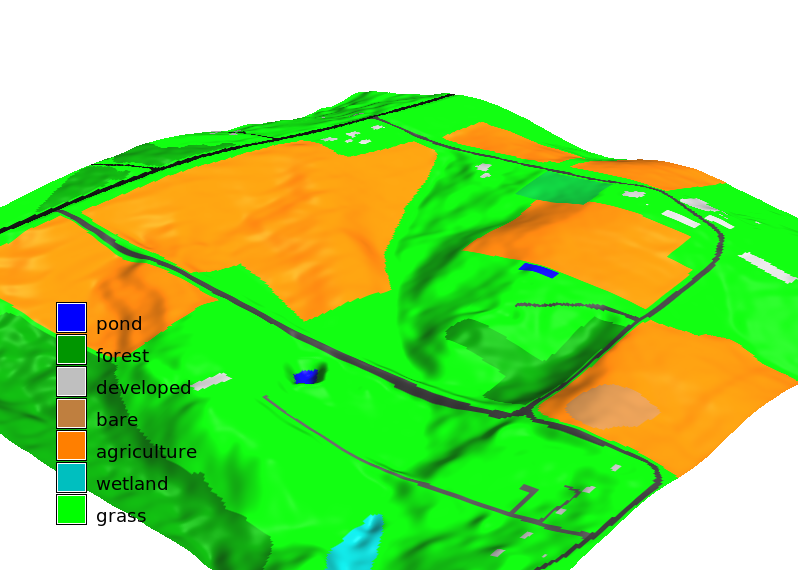
\includegraphics[width=\textwidth]{./images/edu/secref}%

\end{columns}

\bigskip

Listing only geospatial courses where presentation authors are involved.

\end{frame}

%%%%%%%%%%%%%%%%%%%%%%%%%%%%%%%%%%%%%%%%%%%%%%%%%%%%%%%%%%%%%%%%%%%%
\begin{frame}{\coursesTitle}

\begin{columns}[c]

\column{.65\textwidth}

\begin{block}{\href{http://courses.ncsu.edu/mea592/common/}%
  {Multidimensional Geospatial Modeling}}

\begin{itemize}
 \item software:
 \begin{itemize}
   \item \href{http://grass.osgeo.org}{GRASS GIS}
   {\scriptsize
    often with new features such as
    \href{http://grass.osgeo.org/grass70/manuals/temporalintro.html}{Temporal Framework}
    (\href{http://grass.osgeo.org/grass7/}{GRASS GIS 7})
   }
  \item + whatever the students need, e.g.~%
    \href{http://oss.deltares.nl/web/xbeach/}{XBeach}, \href{http://www.liblas.org/}{libLAS}
    or LAStools
 \end{itemize}

%  \item PhD students and highly skilled MS students
%  \item half of the course led by students% (supported by instructor)
 \item curriculum depends on students projects
 \item new technologies:
   \href{http://geospatial.ncsu.edu/osgeorel/tangible-landscape.html}%
   {Tangible Landscape},
   \href{https://www.lib.ncsu.edu/spaces/teaching-and-visualization-lab}%
           {NCSU Hunt Lib Teaching and Vis Lab},
   eye tracking

\end{itemize}

\end{block}

\column{.3\textwidth}

\href{https://www.youtube.com/channel/UCc37pVh-WE46Xkqeq-KZQsA}{%
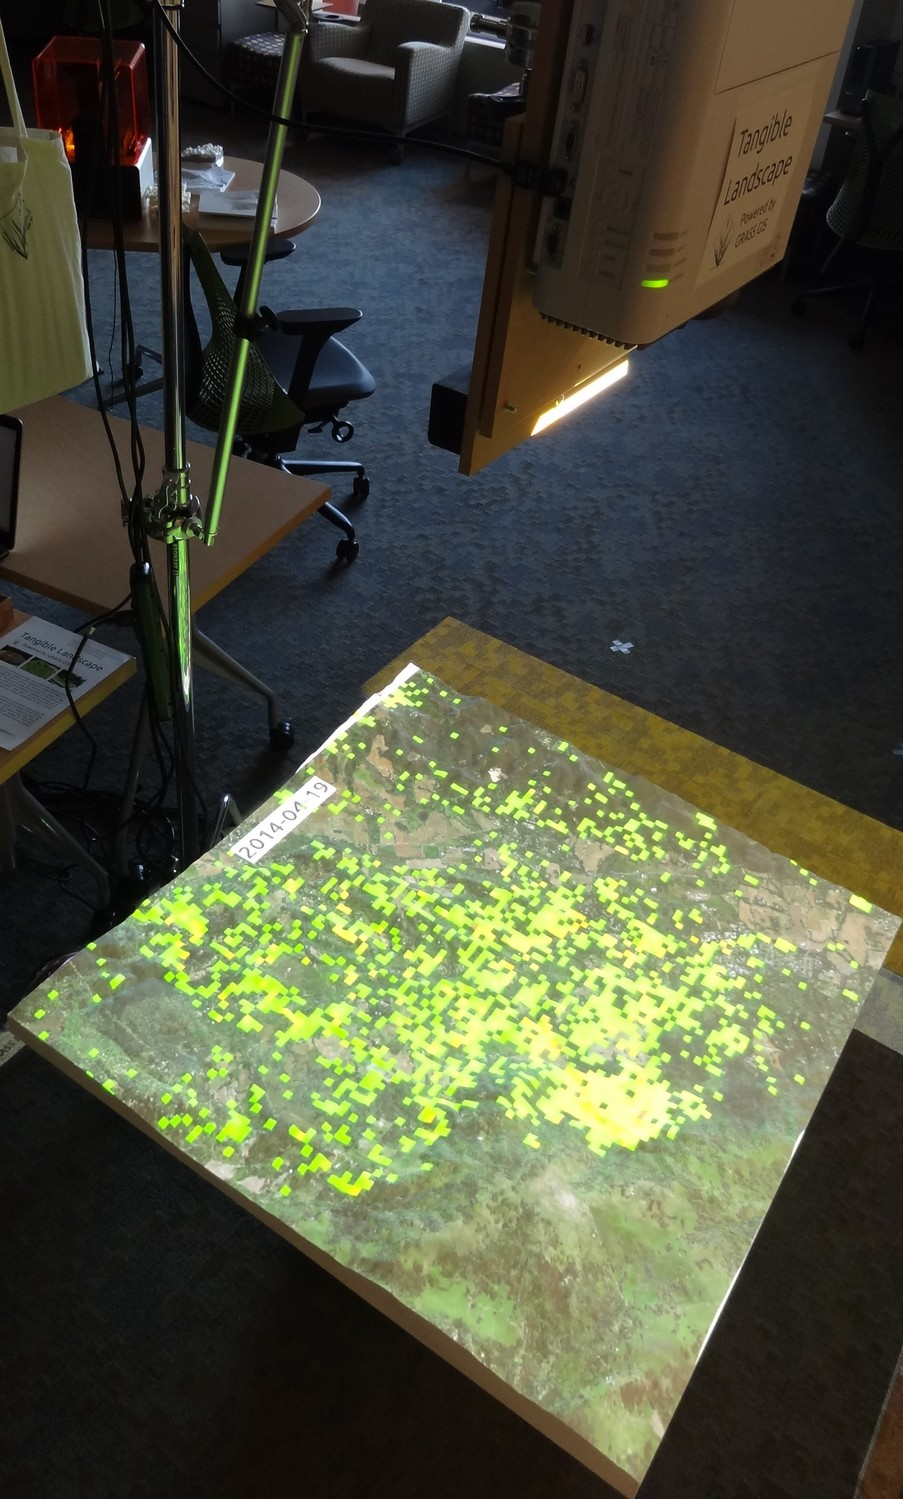
\includegraphics[height=0.65\textheight]{./images/edu/tangible}%
}

\end{columns}

\href{https://www.lib.ncsu.edu/stories/large-scale-visualization-geospatial-data}{%
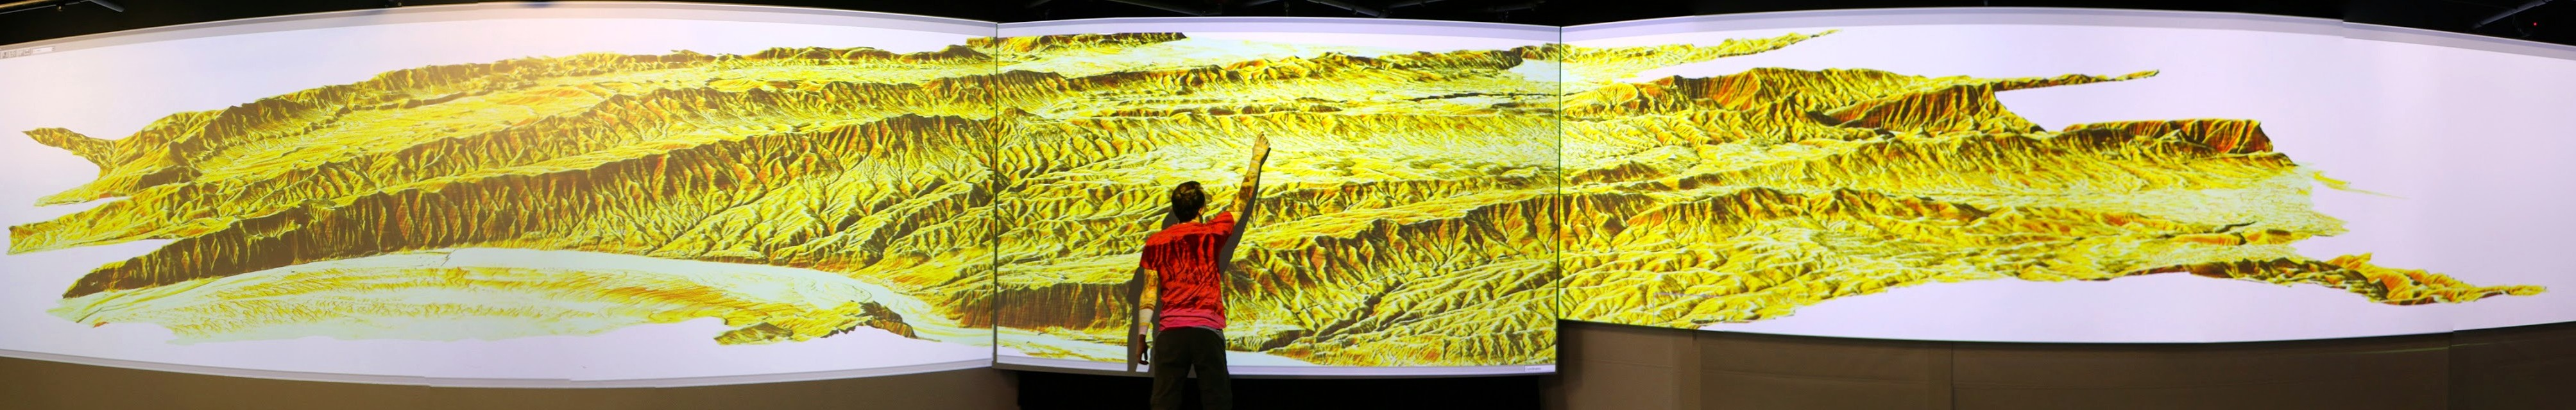
\includegraphics[width=\textwidth]{./images/edu/hunt_vis}%
}

\end{frame}

%%%%%%%%%%%%%%%%%%%%%%%%%%%%%%%%%%%%%%%%%%%%%%%%%%%%%%%%%%%%%%%%%%%%%
\begin{frame}{\coursesTitle}


\begin{columns}[c]

\column{.65\textwidth}

\begin{block}{\href{http://courses.ncsu.edu/lar582/common/}%
  {GIS for Designers}}
\begin{itemize}
 \item software in class:
 \begin{itemize}
  \item ArcGIS
  \item GRASS GIS
  \item Rhino (Rhinoceros)
 \end{itemize}
 \item for projects architects and designers combine a lot of tools
 \begin{itemize}
  \item \href{http://geospatial.ncsu.edu/osgeorel/tangible-landscape.html}{Tangible Landscape}
    (powered by GRASS GIS) was one of them
 \end{itemize}

\end{itemize}

\end{block}

\column{.3\textwidth}

\href{https://www.lib.ncsu.edu/stories/re-imagining-lake-raleigh-woods}{%
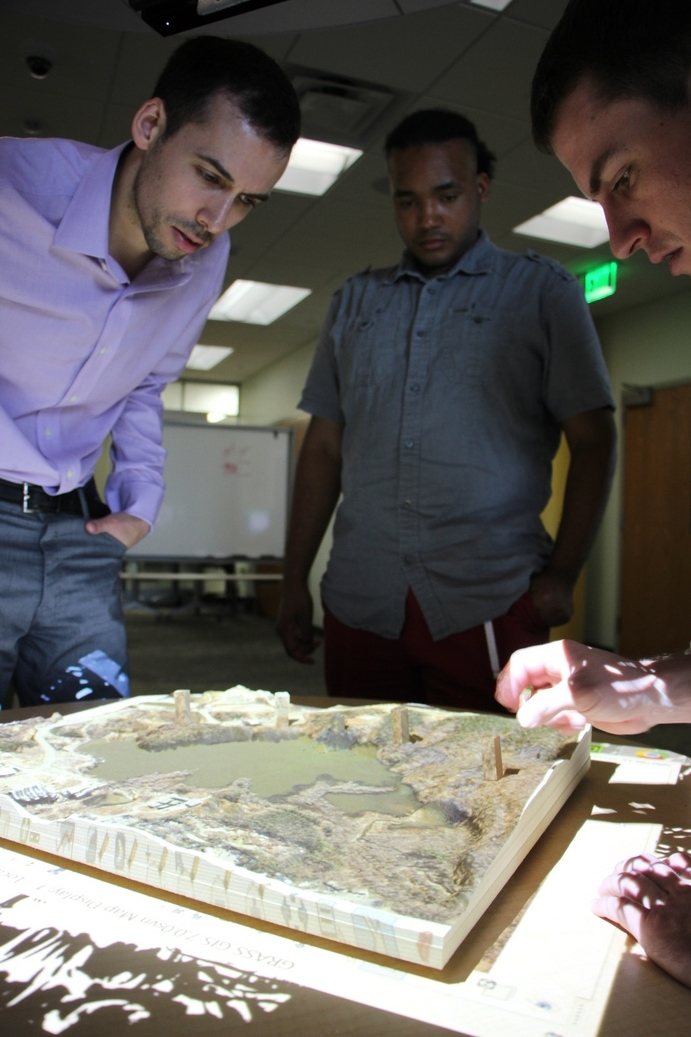
\includegraphics[width=\textwidth]{./images/edu/designers}%
}

\end{columns}

\end{frame}

%%%%%%%%%%%%%%%%%%%%%%%%%%%%%%%%%%%%%%%%%%%%%%%%%%%%%%%%%%%%%%%%%%%%%
\begin{frame}{\coursesTitle}


\begin{block}{\href{http://ncsu-osgeorel.github.io/uav-lidar-analytics-course/}%
  {UAV/lidar Data Analytics}}
\begin{itemize}
 \item under development for this fall semester
 \item Agisoft PhotoScan in class, \href{http://opendronemap.org/}{OpenDroneMap} in projects
\end{itemize}

Related talk: \href{http://europe.foss4g.org/2015/Program}%
                 {Flow analysis using sUAS and lidar data (Helena Mitasova)}
%, Day 3, July 17th, 3:15 PM)

\end{block}

\begin{columns}[c]

\column{.45\textwidth}
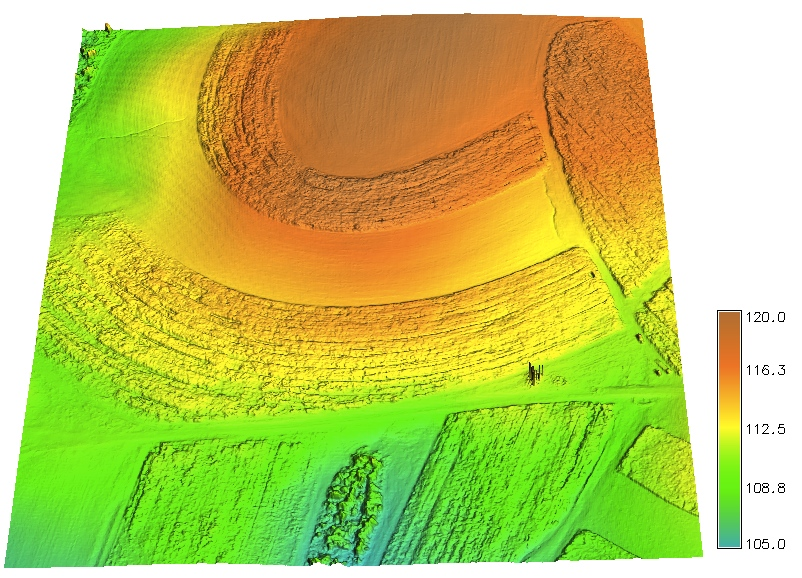
\includegraphics[height=0.5\textheight]{./images/edu/dem}
\column{.45\textwidth}
\hspace{0.2\textwidth}
\rotatebox{-90}{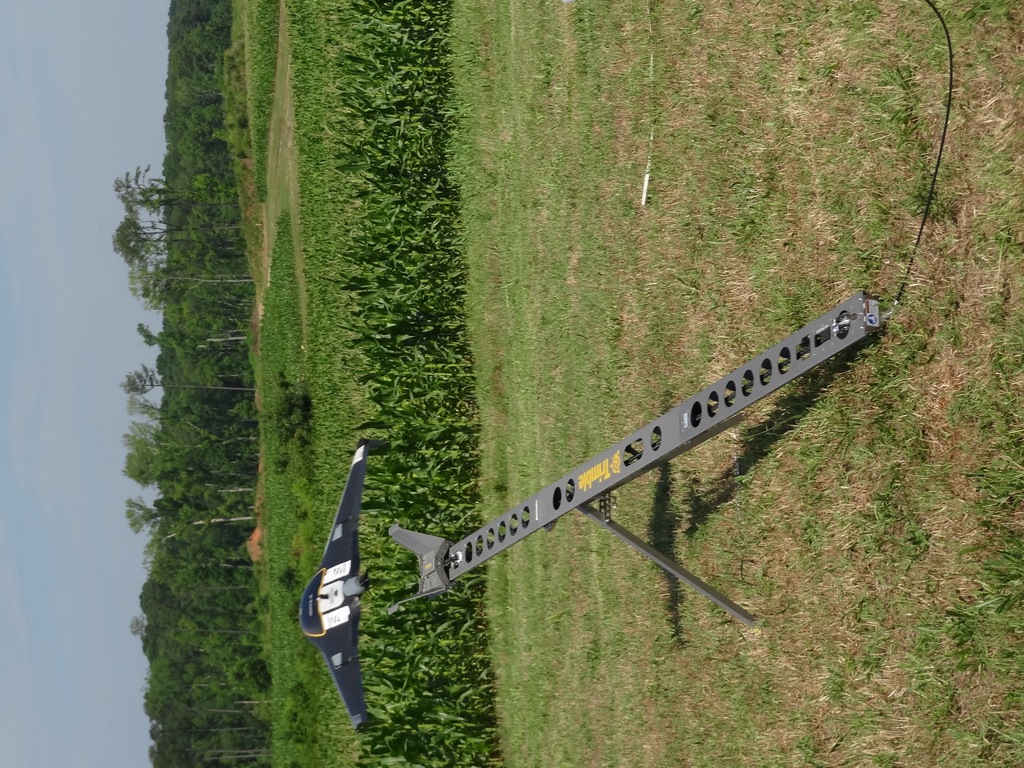
\includegraphics[width=0.5\textheight]{./images/edu/uav}}
\end{columns}

\end{frame}


%%%%%%%%%%%%%%%%%%%%%%%%%%%%%%%%%%%%%%%%%%%%%%%%%%%%%%%%%%%%%%%%%%%%%
\begin{frame}{The idea}

\begin{columns}[c]

\column{.45\textwidth}

\begin{itemize}
 \item lectures:
 \begin{itemize}
  \item theory, concepts
  \item software-independent
 \end{itemize}
 \item labs and assignments:
 \begin{itemize}
  \item relate to given lecture
  \item hands-on, practical
  \item students use software
%   \item software-dependent
 \end{itemize}
\end{itemize}

\column{.45\textwidth}

\bigskip

\centering

\includegraphics[width=0.5\textwidth]{./images/general/bulp}%
\\
\tiny
\color{gray}
Image credit: \href{https://openclipart.org}{Openclipart}

\end{columns}

\end{frame}


%%%%%%%%%%%%%%%%%%%%%%%%%%%%%%%%%%%%%%%%%%%%%%%%%%%%%%%%%%%%%%%%%%%%%
\begin{frame}{The problem}

% Students use software in labs and for assignments.

% In labs and for assignments are software-dependent.

\begin{itemize}
 \item students are becoming (only) software users instead of scientists
 \item students mix software details and general concepts
 \begin{itemize}
  \item saying Shapefile or feature class instead of
    \href{http://www.opengeospatial.org/ogc/glossary/v}{\emph{vector}} data%
    % http://www.opengeospatial.org/ogc/glossary/v
    % http://www.opengeospatial.org/ogc/glossary/f
    % http://www.opengeospatial.org/ogc/glossary/s
    % http://www.opengeospatial.org/ogc/glossary/r
    \ldots
\end{itemize}
 \item bonding with software limits flexibility
 \item software promotes software/vendor-specific formats/technologies
 \item single software choice limits explored algorithms

\end{itemize}

\end{frame}


%%%%%%%%%%%%%%%%%%%%%%%%%%%%%%%%%%%%%%%%%%%%%%%%%%%%%%%%%%%%%%%%%%%%%
\begin{frame}{The solution}

\begin{itemize}
 \item lectures:
 \begin{itemize}
  \item theory, concepts
  \item software-independent
 \end{itemize}
 \item labs and assignments:
 \begin{itemize}
  \item relate to given lecture
  \item hands-on, practical
  \item \alert<1>{students use two different software packages}\pause, in our case:
  \begin{itemize}
   \item GRASS GIS (free and open source)
   \item ArcGIS (proprietary)
  \end{itemize}
 \end{itemize}
  \pause
  \item similar task in both
%   \item students see two different examples of one workflow
  \item opportunity to see what is a general concept
        and what is specific to a~particular software
%   \item they gain flexibility to choose optimal solutions for their future work
\end{itemize}

\end{frame}


%%%%%%%%%%%%%%%%%%%%%%%%%%%%%%%%%%%%%%%%%%%%%%%%%%%%%%%%%%%%%%%%%%%%%
\begin{frame}{Teaching materials}

\begin{itemize}
 \item file format
 \begin{itemize}
  \item originally HTML
  \item selecting new one
  \begin{itemize}
   \item Markdown, missing general standard
   \item reStructuredText, hot candidate
  \end{itemize}
  \item result: HTML (same as delivery format)
  \item presentation slides in HTML5 (\href{http://lab.hakim.se/reveal-js}{Reveal.js})
 \end{itemize}
 \item license: \href{https://creativecommons.org/licenses/by-sa/4.0/}{CC BY-SA}
 \item Git (GitHub hosted)
  {\scriptsize for revision control, collaboration and sharing source code}
 \item registered in \href{http://www.osgeo.org/educational_content}{OSGeo Educational Content Inventory}
\end{itemize}

\href{http://geospatial.ncsu.edu/osgeorel/courses.html}%
  {
  \begin{minipage}[b]{0.2\textwidth}
    \begin{center}
      
\includegraphics[height=0.9\textwidth]{./images/edu/osgeorel_courses_qr}\\
      \tiny \tt geospatial.ncsu.edu/\\osgeorel/courses.html
    \end{center}
  \end{minipage}
  }
\hfill%
\href{http://courses.ncsu.edu/gis582/common/grass/data_models.html}{%
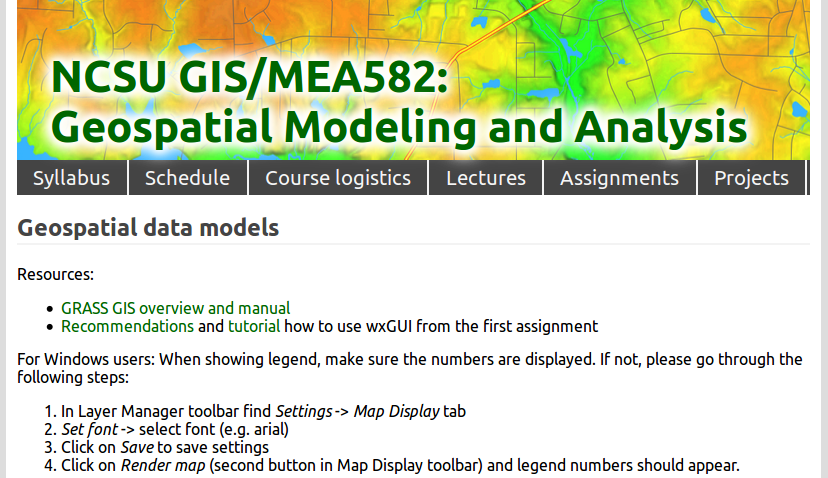
\includegraphics[height=0.2\textwidth]{./images/edu/osgeorel_courses_header}
\hfill
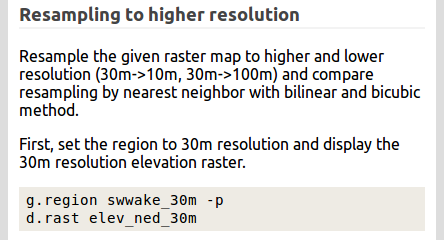
\includegraphics[height=0.2\textwidth]{./images/edu/osgeorel_courses_example}%
}

\end{frame}



%%%%%%%%%%%%%%%%%%%%%%%%%%%%%%%%%%%%%%%%%%%%%%%%%%%%%%%%%%%%%%%%%%%%%
\begin{frame}{GRASS GIS advantage for teaching materials maintenance}

\begin{itemize}
 \item GRASS GIS workflow recorded as commands.
 \begin{itemize}
 \item Screenshots are hard to update while text is easy to update.
 \item GUI dialog filled according to the command.
 \item Commands can be automatically extracted and tested.
 \end{itemize}
\end{itemize}

% \bigskip
% \bigskip
\begin{center}
\colorbox{gray!20}{
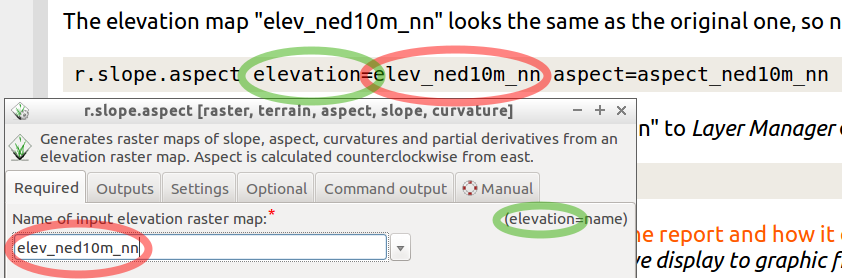
\includegraphics[height=0.5\textheight]{./images/edu/grass_cmd_gui}
}
\end{center}


% \bigskip
% \bigskip

\scriptsize
For ArcGIS we also use just text, but, unlike in GRASS GIS,
the names in dialogs are not part of the API, so they change more often.
{\tiny(Course running since 2008.)}

\end{frame}

%%%%%%%%%%%%%%%%%%%%%%%%%%%%%%%%%%%%%%%%%%%%%%%%%%%%%%%%%%%%%%%%%%%%%
\begin{frame}{Paper}

\href{http://www.mdpi.com/2220-9964/4/2/942}%
  {\emph{Integrating Free and Open Source Solutions into Geospatial Science Education}
  \hfill \footnotesize \color{gray} Open Access}

Vaclav Petras\n{1,\,4},
Anna Petrasova\n{1,\,4},
Brendan Harmon\n{2,\,4},
\mbox{Ross K. Meentemeyer}\n{3,\,4},
and Helena Mitasova\n{1,\,4}

\medskip

{\tiny
$^1$Department of Marine, Earth, and Atmospheric Sciences\\
$^2$Department of Landscape Architecture\\
$^3$Department of Forestry and Environmental Resources\\
$^4$\href{http://cnr.ncsu.edu/geospatial/}{Center for Geospatial Analytics}
and \href{http://geospatial.ncsu.edu/osgeorel/}{NCSU OSGeoREL}
  -- \href{www.geoforall.org}{part of ICA-OSGeo-ISPRS Network (aka \alert{Geo for All})}\\
}{\scriptsize
North Carolina State University, Raleigh, USA\\
}

\medskip

In: \href{http://www.mdpi.com/journal/ijgi/special_issues/science-applications}%
{\emph{ISPRS International Journal of Geo-Information}}. 2015.
% Special Issue "Open Geospatial Science and Applications"

\bigskip

\href{http://dx.doi.org/10.3390/ijgi4020942}%
  {
  \begin{minipage}[b]{0.2\textwidth}
    \begin{center}
      
\includegraphics[height=0.9\textwidth]{./images/edu/paper_qr}\\
      \tiny \tt doi:10.3390/ijgi4020942
    \end{center}
  \end{minipage}
  }
\hfill
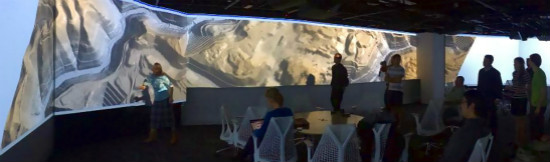
\includegraphics[height=0.2\textwidth]{./images/edu/paper_picture}

\end{frame}


%%%%%%%%%%%%%%%%%%%%%%%%%%%%%%%%%%%%%%%%%%%%%%%%%%%%%%%%%%%%%%%%%%%%%
\begin{frame}[fragile]{Standardized Sample Datasets}

\begin{itemize}
 \item region specific datasets limit sharing of hands-on teaching material
 \item new version of North Carolina
 \begin{itemize}
  \item commonly available data, frequently used in examples
  \item standardized names such as \textit{elevation}, \textit{streets}, or \textit{lakes}
  \begin{itemize}
   \item rather than \textit{srtm}, \textit{dem\_10m}, \textit{streets\_como}
  \end{itemize}
 \end{itemize}
 \item \alert{different datasets should use the same standardized names}
 \item challenges:
 \begin{itemize}
  \item attributes, coordinates, values, extents, resolutions
 \end{itemize}

\end{itemize}

\smallskip

\begin{columns}[c]

 \column{.45\textwidth}
\scriptsize
\begin{verbatim}
g.region raster=elevation
r.relief input=elevation output=shade
\end{verbatim}
\begin{verbatim}
d.shade shade=shade color=elevation
\end{verbatim}
\vfill\hfill\hfill
\href{http://grasswiki.osgeo.org/wiki/GRASS_GIS_Standardized_Sample_Datasets}{%
$\blacktriangleright$ wiki page}

\column{.40\textwidth}
 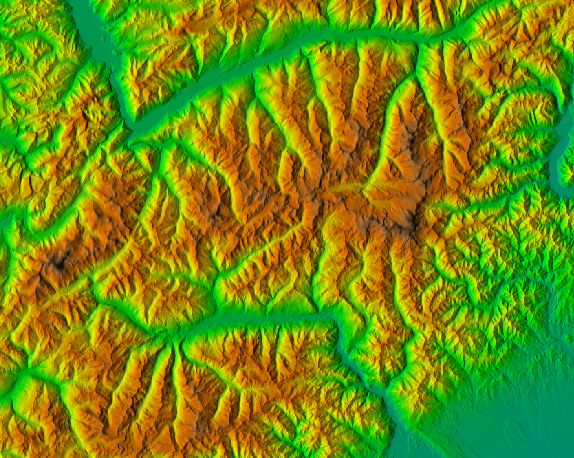
\includegraphics[width=\textwidth]{./images/dataset/std_dataset_piemonte_shaded_elevation}%
\end{columns}


\end{frame}



%%%%%%%%%%%%%%%%%%%%%%%%%%%%%%%%%%%%%%%%%%%%%%%%%%%%%%%%%%%%%%%%%%%%%
\begin{frame}{Standardized Sample Dataset: North Carolina, USA}

\begin{center}
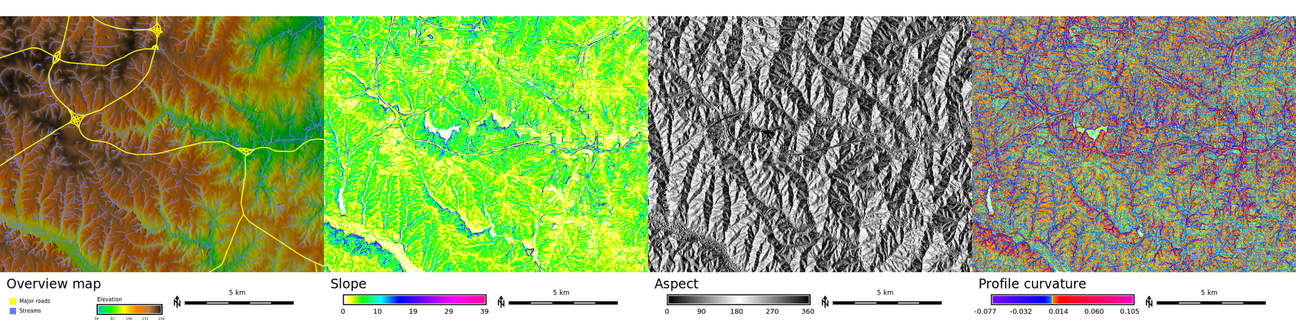
\includegraphics[width=\textwidth]{./images/dataset/std_dataset_nc_stripe.png}
\end{center}


Helena Mitasova\n{1} and Markus Neteler\n{2}, authors of
\mbox{\href{http://grassbook.org/}{\it Open Source GIS: A GRASS GIS Approach}}
{\scriptsize (fourth edition in preparation)}

\bigskip

{\scriptsize
$^1$\href{http://www.meas.ncsu.edu/}%
{Department of Marine, Earth, and Atmospheric Sciences,
North Carolina State University, USA}

$^2$\href{http://gis.cri.fmach.it/}%
% GIS and Remote Sensing Unit
{Research and Innovation Centre, Fondazione Edmund Mach, Italy}
}

\end{frame}

%%%%%%%%%%%%%%%%%%%%%%%%%%%%%%%%%%%%%%%%%%%%%%%%%%%%%%%%%%%%%%%%%%%%%
\begin{frame}{Standardized Sample Dataset: Czech Republic}

\begin{center}
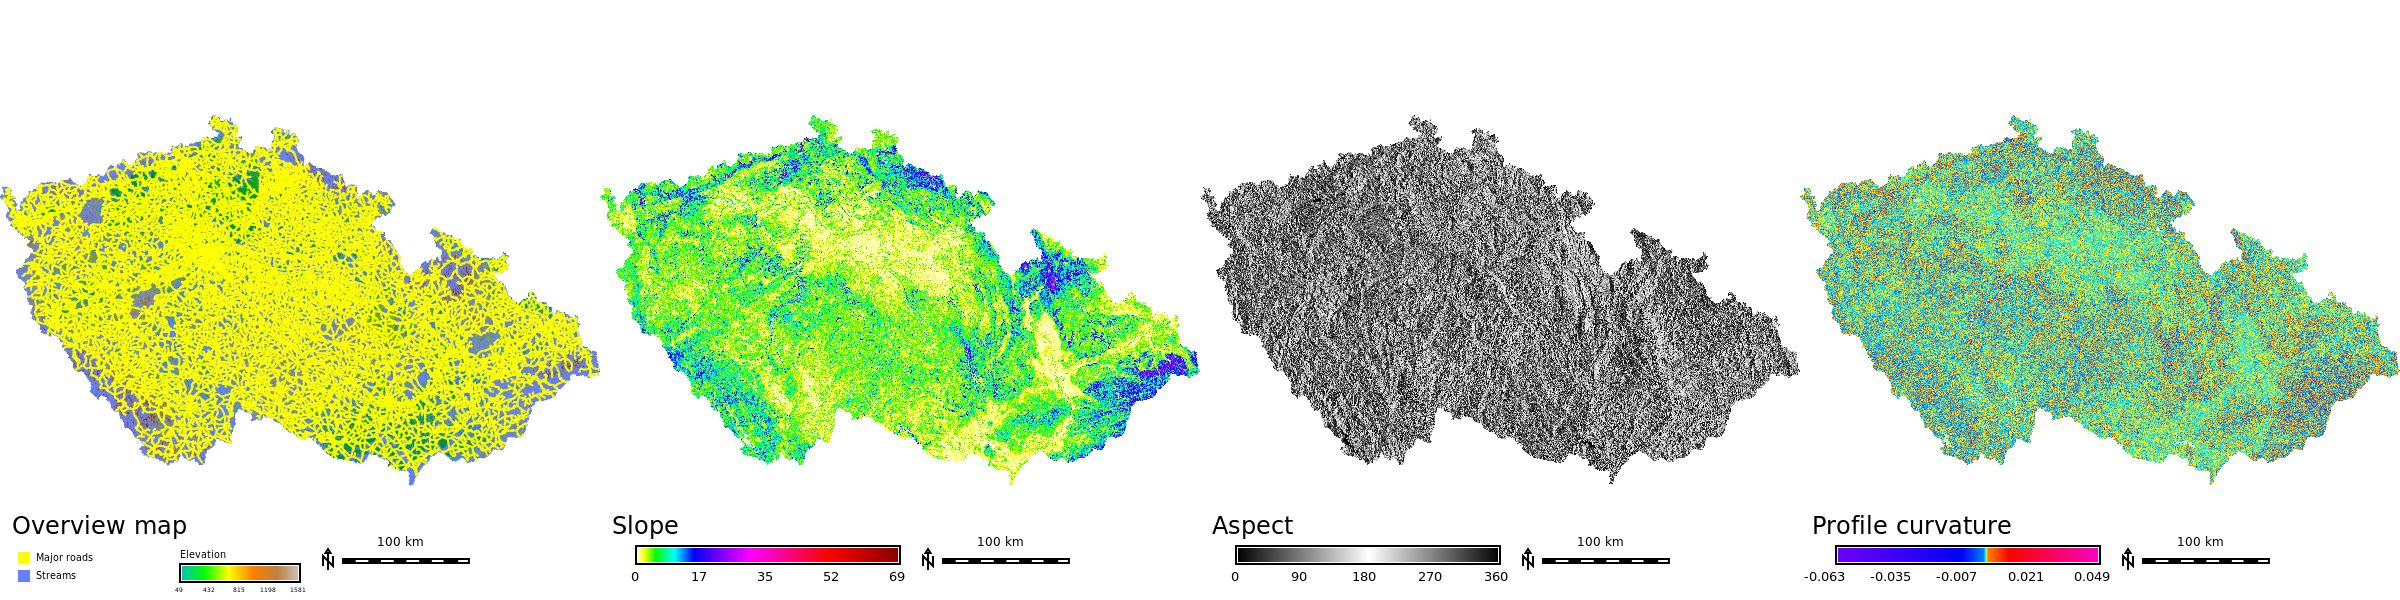
\includegraphics[width=\textwidth]{./images/dataset/std_dataset_cz_stripe.png}
\end{center}

\href{http://gismentors.eu/}{Martin Landa\n{*} and Jachym Cepicky from GISMentors}

\bigskip

$^*$\href{http://geomatics.fsv.cvut.cz/research/osgeorel/}%
{\scriptsize
OSGeoREL
at Czech Technical University in Prague,
Faculty of Civil Engineering
}

\end{frame}

%%%%%%%%%%%%%%%%%%%%%%%%%%%%%%%%%%%%%%%%%%%%%%%%%%%%%%%%%%%%%%%%%%%%%
\begin{frame}{Standardized Sample Dataset: Piedmont, Italy}
% English: Piedmont [ˈpiːdmɒnt] PEED-mont
% Italian: Piemonte [pjeˈmonte]

\begin{center}
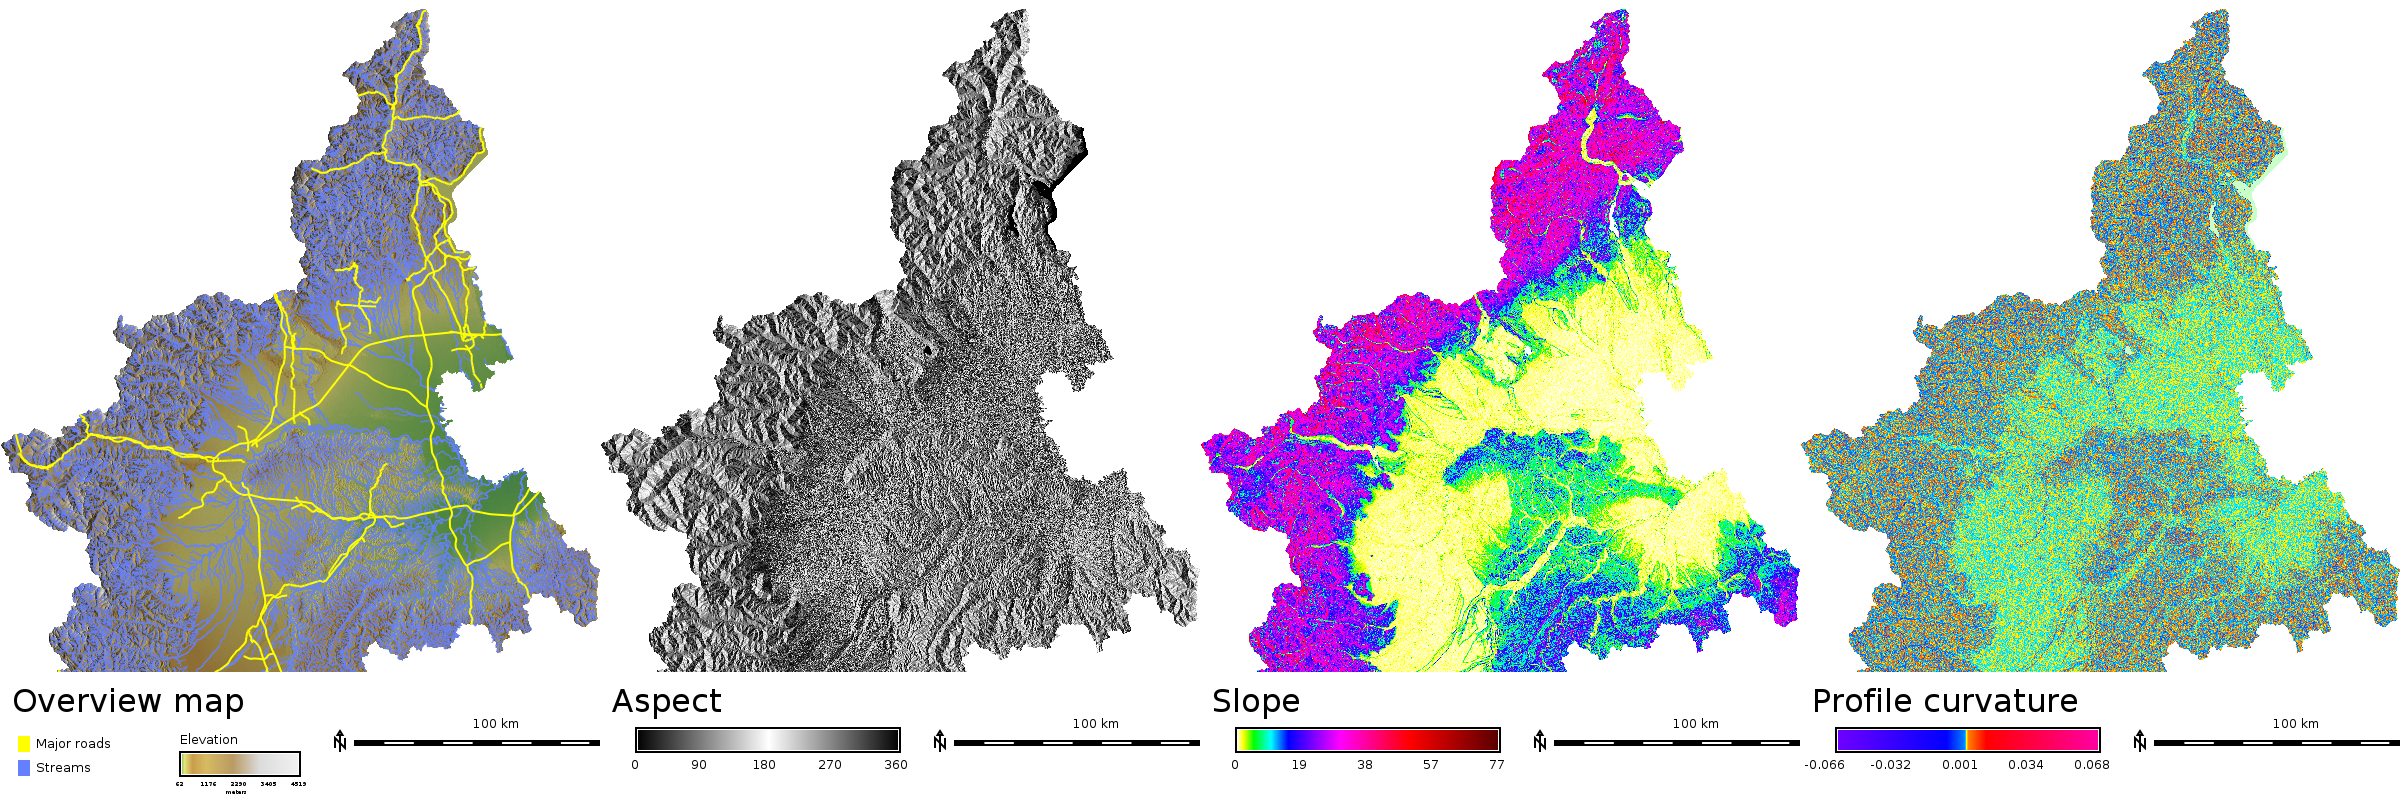
\includegraphics[width=\textwidth]{./images/dataset/std_dataset_it_stripe.png}
\end{center}


Luca Delucchi and Markus Neteler

{\scriptsize
\href{http://gis.cri.fmach.it/}{Research and Innovation Centre, Fondazione Edmund Mach, Italy}
}

\end{frame}

%%%%%%%%%%%%%%%%%%%%%%%%%%%%%%%%%%%%%%%%%%%%%%%%%%%%%%%%%%%%%%%%%%%%%
\begin{frame}{Standardized Sample Dataset: Puerto Rico}

\begin{center}
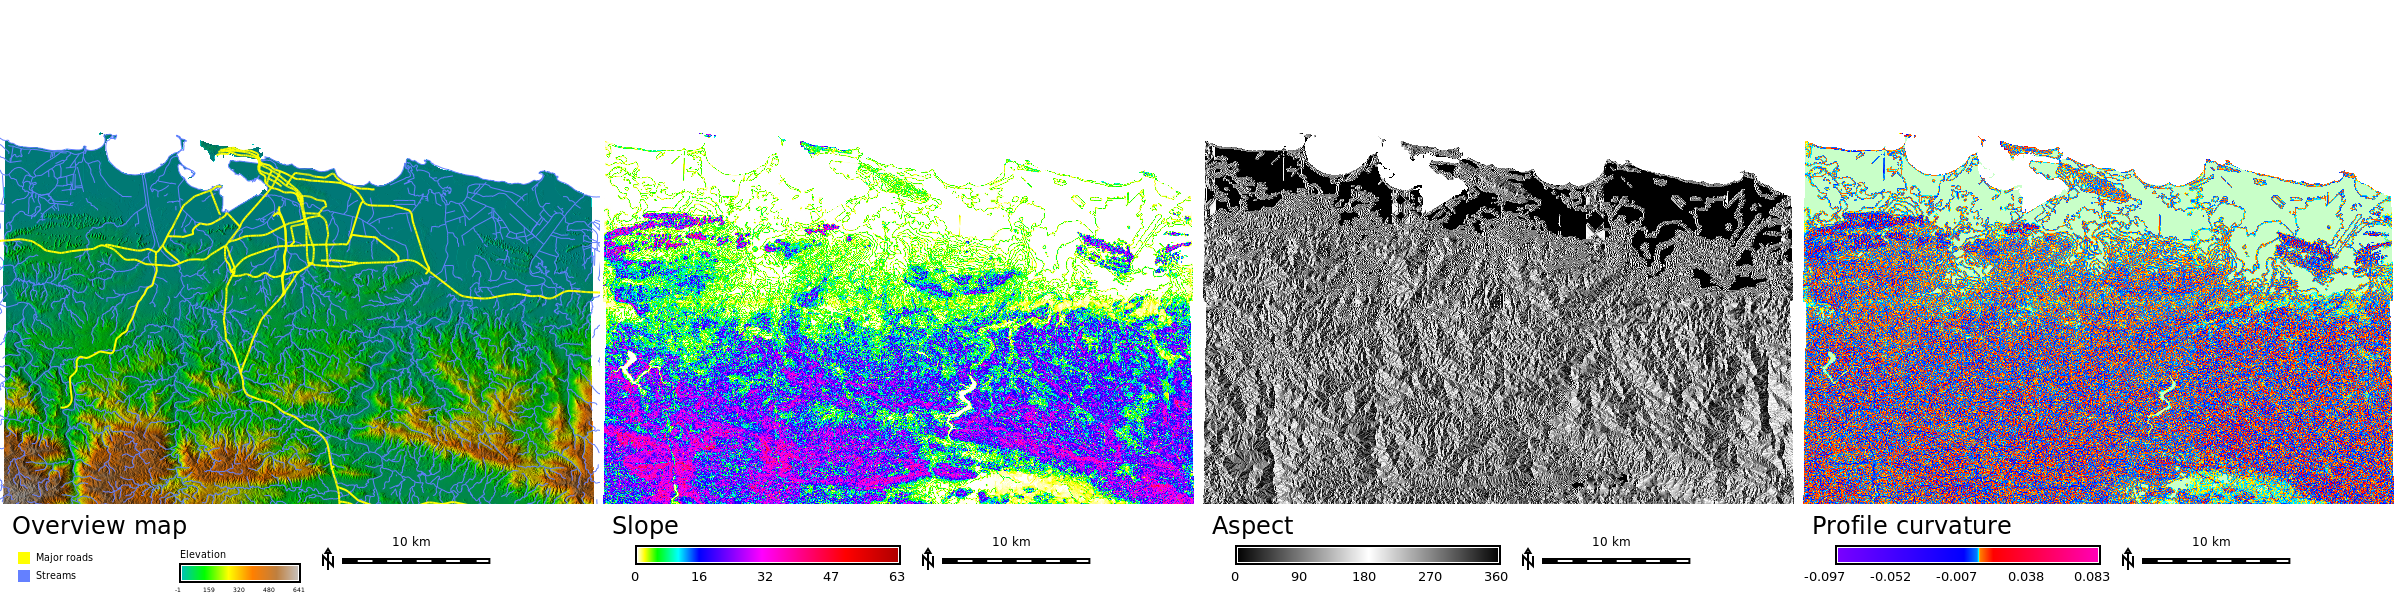
\includegraphics[width=\textwidth]{./images/dataset/std_dataset_pr_stripe.png}
\end{center}

Keren Cepero-Perez

{\scriptsize
\href{http://www.meas.ncsu.edu/}%
{Department of Marine, Earth, and Atmospheric Sciences,
North Carolina State University, USA}
}

\end{frame}


%%%%%%%%%%%%%%%%%%%%%%%%%%%%%%%%%%%%%%%%%%%%%%%%%%%%%%%%%%%%%%%%%%%%%
\begin{frame}{Future directions: IPython Notebook}

Used in workshop \emph{How to write a Python GRASS GIS 7 addon}
\begin{itemize}
 \item \url{https://github.com/wenzeslaus/python-grass-addon}
\end{itemize}


\begin{block}{Solution}
\begin{itemize}
 \item Docker + GRASS GIS + IPython Notebook
 \item Dockerfile:
 \begin{itemize}
  \item \url{https://github.com/wenzeslaus/grass-gis-docker}
 \end{itemize}
\end{itemize}
\end{block}

\centering
\begin{minipage}{0.6\textwidth}
\begin{minipage}[b]{0.45\textwidth}

\includegraphics[width=\textwidth]{./images/logos/ipython}
\vspace{0.1\textwidth}

\includegraphics[width=\textwidth]{./images/logos/docker_dark}
\end{minipage}

\includegraphics[width=0.3\textwidth]{./images/logos/grass_gis}
\end{minipage}

\end{frame}


%%%%%%%%%%%%%%%%%%%%%%%%%%%%%%%%%%%%%%%%%%%%%%%%%%%%%%%%%%%%%%%%%%%%
\begin{frame}{NCSU OSGeoREL workshops and tutorials}

\begin{block}{\href{http://ncsu-osgeorel.github.io/grass-intro-workshop/}%
  {Introduction to GRASS GIS}}
  \footnotesize
  Delivered at NCSU
\end{block}

\begin{block}{\href{http://ncsu-osgeorel.github.io/grass-temporal-workshop/}%
  {Spatio-temporal data handling and visualization in GRASS GIS}}
  \footnotesize
  FOSS4G 2014 (Portland) workshop, also delivered at NCSU
\end{block}


\begin{block}{\href{http://ncsu-osgeorel.github.io/erosion-modeling-tutorial/}%
  {Soil erosion and deposition modeling}}
  \footnotesize
  Part of a broader project; workflows for GRASS GIS and ArcGIS
\end{block}


\begin{block}{\href{https://github.com/wenzeslaus/python-grass-addon}%
  {How to write a Python GRASS GIS 7 addon}}
  \footnotesize
  FOSS4G Europe 2015 (Como) workshop, also delivered at NCSU
\end{block}

\bigskip
% \footnotesize
\alert{Workshops are a way how to experiment with what to teach and how.}

\end{frame}


%%%%%%%%%%%%%%%%%%%%%%%%%%%%%%%%%%%%%%%%%%%%%%%%%%%%%%%%%%%%%%%%%%%%%
% \begin{frame}{Future directions: Educate educators}
% 
% \begin{itemize}
%   \item instructors involvement in community is more important then students in involvement community
% \end{itemize}
% 
% \end{frame}

%%%%%%%%%%%%%%%%%%%%%%%%%%%%%%%%%%%%%%%%%%%%%%%%%%%%%%%%%%%%%%%%%%%%%
\begin{frame}{Future directions: Tools for open science course}

\begin{overlayarea}{\textwidth}{\textheight}

\begin{itemize}
 \item Course dedicated to
 \begin{itemize}
  \item exploring important role FOSS plays in science
  \item overview of tools and methods common in FOSS and desperately needed in science
  \item open access, open data, open standards, open...
  \item reusability and reproducibility are standard in FOSS
 \end{itemize}
\end{itemize}

\smallskip

\centering

\includegraphics[height=0.5\textheight]{./images/general/open_up_book}%
\\
\tiny
Image credit: \href{https://opensource.com/}{Opensource.com}


\end{overlayarea}

\end{frame}


%%%%%%%%%%%%%%%%%%%%%%%%%%%%%%%%%%%%%%%%%%%%%%%%%%%%%%%%%%%%%%%%%%%%%
\begin{frame}{Future directions: Software, technologies and platforms}

\begin{itemize}
 \item \href{http://openstreetmap.org/}{OpenStreetMap},
    \href{http://teachosm.org}{TeachOSM}, \href{http://learnosm.org}{LearnOSM}
 \begin{itemize}
  \item for introduction to geography or GIS
  \item as an example of community-based project
  \item as data source in advanced courses
 \end{itemize}
 \item \href{http://mapstory.org/}{MapStory} {\scriptsize for student projects}
 \item \href{http://imincik.github.io/gis-lab/}{GIS.lab} {\scriptsize for easy lab setup}
 \item \href{http://jupyter.org/}{IPython/Jupyter},
    \href{https://github.com/jupyter/jupyterhub}{JupyterHub},
    \href{https://github.com/jupyter/tmpnb}{tmpnb}
 \item
    desktop to browser:
    \href{https://developer.gnome.org/gtk3/stable/gtk-broadway.html}{GTK+ Broadway},
    \href{https://kanaka.github.io/noVNC/}{noVNC}
    {\tiny (to get something like \href{https://www.rollapp.com/}{rollApp})}
 \item web-based tool to explore algorithm behavior in teaching materials
 \item link teaching materials, standard user manual and the source code
\end{itemize}

\end{frame}

%%%%%%%%%%%%%%%%%%%%%%%%%%%%%%%%%%%%%%%%%%%%%%%%%%%%%%%%%%%%%%%%%%%%%
\begin{frame}{}

\begin{block}{Summary}
 \begin{itemize}
  \item \href{http://dx.doi.org/10.3390/ijgi4020942}%
    {improve students' geospatial skills by teaching 2 software packages}
  \item \href{http://dx.doi.org/10.3390/ijgi4020942}%
    {use available tools like Git and HTML to create teaching materials}
  \item \href{http://grasswiki.osgeo.org/wiki/GRASS_GIS_Standardized_Sample_Datasets}%
    {create a dataset with standardized names for your region}
 \end{itemize}

\end{block}

\bigskip

\centering
\href{https://github.com/wenzeslaus/foss-in-geospatial-science-education}{%

\includegraphics[width=0.2\textwidth]{./images/general/slides_qr}\\%
\texttt{github.com/wenzeslaus/foss-in-geospatial-science-education}%
}

\end{frame}

\end{document}
